% !TEX root = ../main.tex
\section{Introduction}
\label{sec:intro}

Detection and identification using artificial landmarks, known as fiducial markers, has long been used in augmented reality and computer vision applications. Over the last decade, there have been numerous marker systems, such as ARTags, Apriltags, and Rune Tags, designed to improve detection encoding precision. However, these systems are not robust enough to be used reliability in many robotic applications.

Compared to markerless detection algorithms, fiducial marker methods are simpler and more consistent. They yield great results in computer vision tasks that require high detection accuracy like camera calibrations and 3D reconstruction. Furthermore, the fiducial tags have gained popularity in the robotic community for having unique characteristics of high detection rates and numerous encoding schemes. For example, Apriltags are commonly used to test SLAM systems, or finding ground truth for objects in manipulation and motion planning tasks as shown in Figure \ref{fig:table_clearing}. 

However, obtaining highly accurate pose estimations using fiducial tags from noisy data remains a challenge. This is especially important for robotic applications because small errors can cause large system failures as the errors propagate and amplify through the system. Currently, the fiducial tag systems yield good results under well conditioned or rendered environments, but this does not translate to ill-conditioned settings. For instance, when Apriltags, a state of the art fiducial marker, are used with low resolution cameras or harsh lighting conditions, the system often produces poses with tremendous rotational errors as shown in Figure \ref{fig:mismatch}. In fact, we observe that the localization accuracy of the Apriltag system perform significantly worse when there is noise in the captured image. This is a difficult problem because RGB sensors are often sensitive to lighting, and current fiducial systems are not designed to take advantage of other sensors commonly available on robots.


\begin{figure}[h]
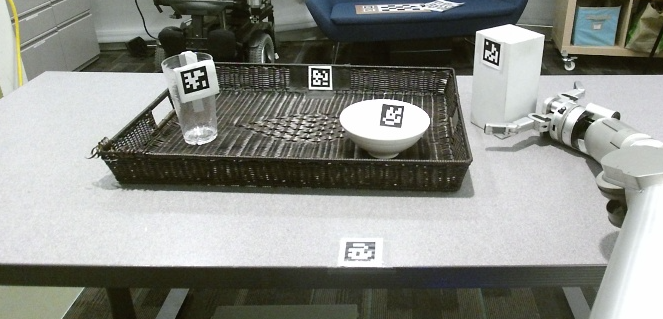
\includegraphics[width=\columnwidth, height=120px]{figs/table_clearing_rgb_small} \\
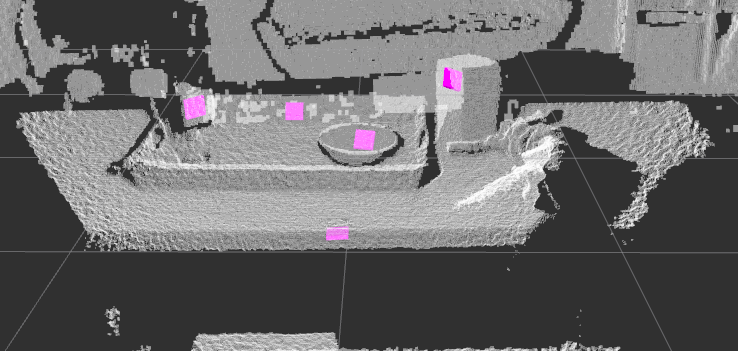
\includegraphics[width=\columnwidth, height=120px]{figs/table_clearing_depth}
\label{fig:table_clearing}
\caption{Apriltags are used to find groundtruth poses of different objects in manipulation tasks}
\end{figure}

We present two main contributions in this paper. First, we conducted an in-depth analysis on the effect of various noises on the pose estimation process. In particular, the noise in RGB images creates a perspective ambiguity problem that makes the pose estimation challenging without additional information. Second, we describe a novel method that takes advantage of the RGBD sensors that are commonly available on most robotic systems to accurately estimate the pose from a single tag under noisy conditions in real time. In the core of the algorithm, we recognize that RGB and depth sensors work optimally under different conditions. Therefore, their strength can be combined meaningfully to improve the localization accuracy under difficult conditions. There are a few key features to this algorithm: 
\begin{itemize}
\item This method is highly robust to noise in the scene. It can obtain accurate poses suitable for a wide range robotic applications.   
\item It is easily generalizable to most fiducial tag designs.
\item It has very small computation overhead, and can be ran in real time. 
\end{itemize}

This paper also presents empirical results demonstrating the successful performance of the algorithm on captured data from a humanoid robot. Our implementation of the algorithm is based off of the Apriltag detection pipeline and it is integrated with ROS. 